%
% management.tex
%
% Copyright (C) 2021 by SpaceLab.
%
% FloripaSat-2 Documentation
%
% This work is licensed under the Creative Commons Attribution-ShareAlike 4.0
% International License. To view a copy of this license,
% visit http://creativecommons.org/licenses/by-sa/4.0/.
%

%
% \brief Mission management chapter.
%
% \author Gabriel Mariano Marcelino <gabriel.mm8@gmail.com>
%
% \institution Universidade Federal de Santa Catarina (UFSC)
%
% \version 0.2.0
%
% \date 2021/07/15
%

\chapter{Mission Management} \label{ch:management}

\section{Requirements}

\begin{enumerate}
    \item The power system shall be able to harvest solar energy.
    \item The power system shall be able to store energy for use when FloripaSat-2 is eclipsed.
    \item The power system shall supply energy to all other modules.
    \item The data handling system shall communicate with the other modules and store their data.
    \item The communications system shall send a beacon signal periodically using VHF radio.
    \item The communications system shall send the CubeSat telemetry using UHF radio.
    \item The communications system shall be able to receive telecommands and respond to them accordingly.
    \item The attitude system shall be able to perform a 1-axis stabilization of the CubeSat.
    \item FloripaSat-2 shall have the capability to receive and execute a shutdown telecommand, therefore ceasing all transmissions.
    \item The downlink transmissions shall be done once at a time, either telemetry or beacon.
    \item The ground station shall operate under the proper radio frequency communication licenses.
    \item FLoripaSat-2 shall comply with international and Brazilian radio license agreements and restrictions.
    \item The team shall build and operate a ground station for full communication with FloripaSat-2.
\end{enumerate}

\section{Schedule}

\begin{table}[!h]
    \centering
    \begin{tabular}{cC{0.6cm}C{0.6cm}C{0.6cm}C{0.6cm}C{0.6cm}C{0.6cm}C{0.6cm}C{0.6cm}C{0.6cm}C{0.6cm}C{0.6cm}C{0.6cm}}
        \toprule[1.5pt]
        \multirow{3}{*}{\textbf{Activity}} & \multicolumn{12}{c}{\textbf{Month (2021)}} \\
                                           & Jan & Feb & Mar & Apr & May & Jun & Jul & Aug & Sep & Oct & Nov & Dez \\
        \midrule
        1                                  & \fc & \fc & \fc & \fc &     &     &     &     &     &     &     &     \\
        2                                  & \fc & \fc & \fc & \fc &     &     &     &     &     &     &     &     \\
        3                                  & \fc & \fc & \fc & \fc & \fc & \fc & \fc & \fc & \fc &     &     &     \\
        4                                  & \fc & \fc & \fc & \fc & \fc & \fc &     &     &     &     &     &     \\
        5                                  &     &     &     & \fc & \fc & \fc & \fc & \fc & \fc & \fc &     &     \\
        6                                  &     &     &     &     & \fc & \fc & \fc & \fc & \fc & \fc & \fc &     \\
        7                                  &     &     &     &     &     &     &     & \fc & \fc & \fc &     &     \\
        8                                  &     &     &     &     &     &     &     & \fc & \fc & \fc & \fc &     \\
        9                                  &     &     &     &     &     &     &     &     & \fc & \fc & \fc & \fc \\
        10                                 &     &     &     &     &     &     &     &     &     & \fc & \fc &     \\
        11                                 &     &     &     &     &     &     &     &     &     & \fc & \fc &     \\
        12                                 &     &     &     &     &     &     &     &     &     &     & \fc &     \\
        13                                 &     &     &     &     &     &     &     &     & \fc & \fc & \fc & \fc \\
        14                                 &     &     &     &     &     &     &     &     &     &     & \fc & \fc \\
        \bottomrule[1.5pt]
    \end{tabular}
    \caption{Mission schedule.}
    \label{tab:mission-schedule}
\end{table}

Each activity of \autoref{tab:mission-schedule} is decribed below:

\begin{enumerate}
    \item Acquisition and manufacturing of critical elements and components for the solo platform.
    \item Acquisition and manufacture of elements and components critical to the payload.
    \item Acquisition and manufacturing of critical elements and components for the solo segment.
    \item Compatibility tests between platform and payload in SpaceLab UFSC.
    \item Integration of the engineering model in SpaceLab UFSC.
    \item Preparation and suitability of the ground segment.
    \item Verification and validation of the engineering model at SpaceLab UFSC.
    \item Verification and validation of the flight model at SpaceLab UFSC.
    \item Data collection platforms installation.
    \item Verification and validation tests of Engineering Model compatibility with EMMN in the INPE / CRN in Natal.
    \item Environmental tests at the Integration and Testing Laboratory (LIT/INPE).
    \item Flight model acceptance and ground segment review.
    \item Ground segment delivery.
    \item Flight model delivery.
\end{enumerate}

\section{Product Tree}

\begin{figure}[!ht]
    \begin{center}
        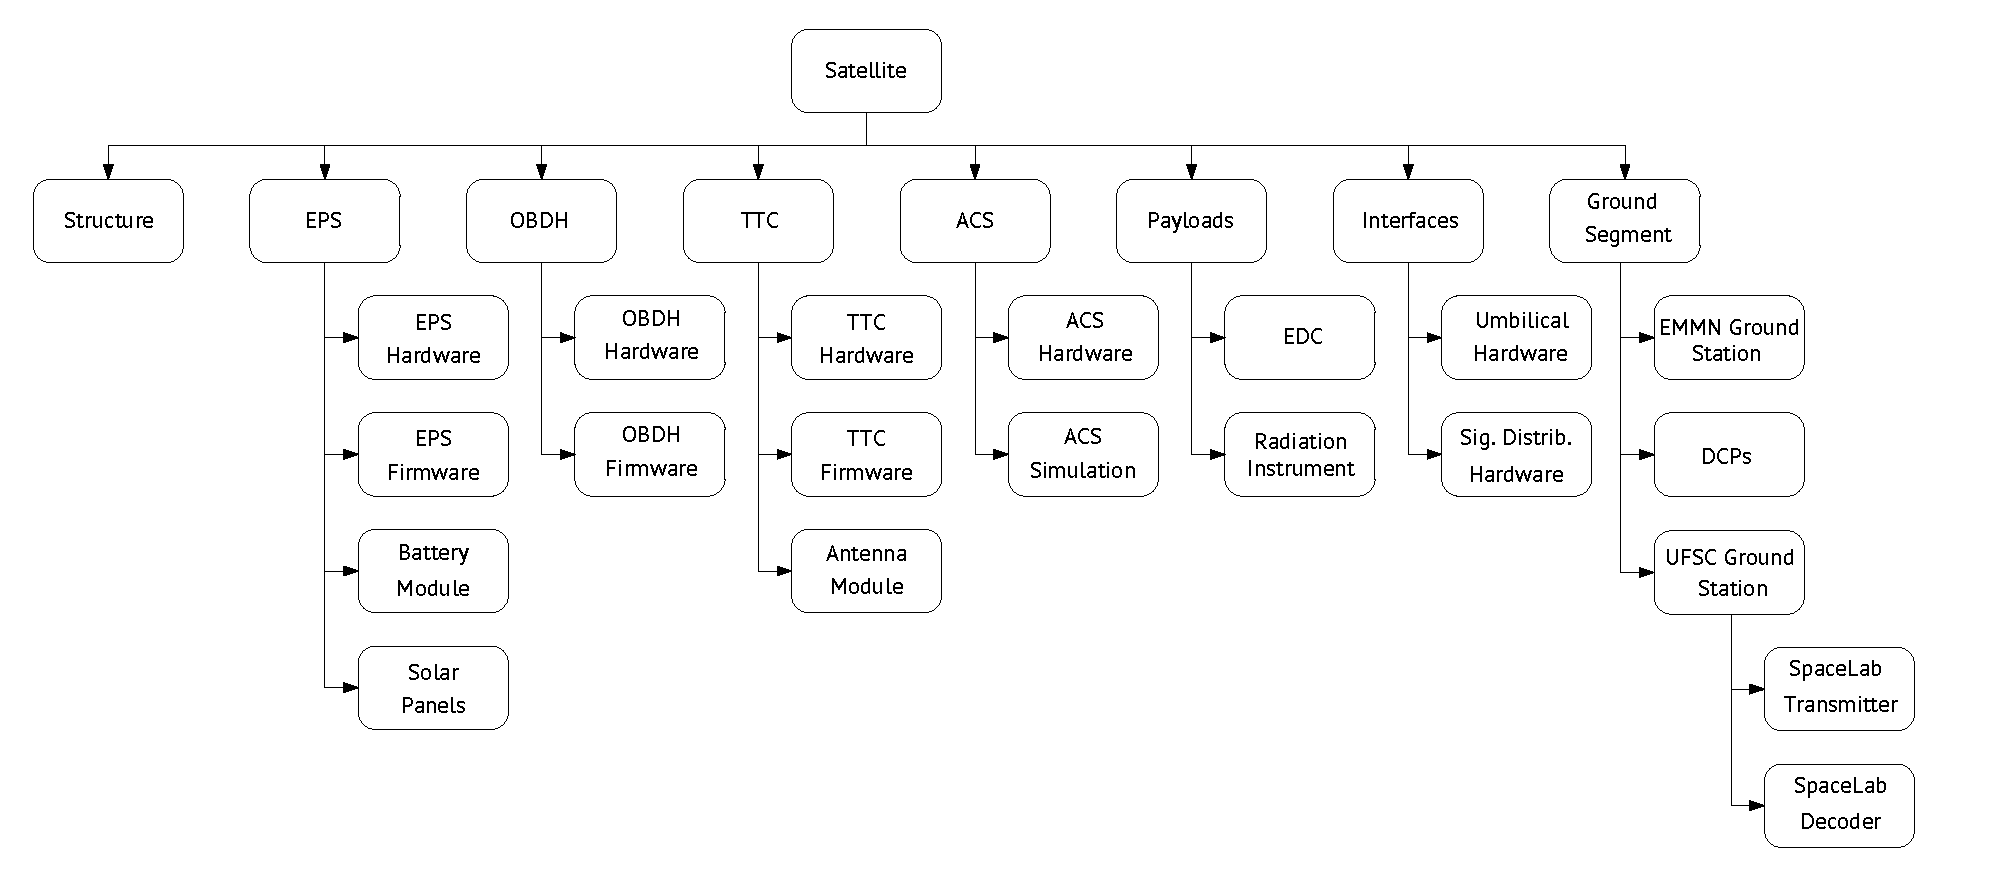
\includegraphics[width=\textwidth]{figures/product-tree.pdf}
        \caption{Product tree of the satellite.}
        \label{fig:product-tree}
    \end{center}
\end{figure}

\subsection{Working Breakdown Structure}

The Working Breaking Structure (WBS\nomenclature{\textbf{WBS}}{\textit{Working Breakdown Structure.}}) is presented as a diagram in \autoref{fig:wbs}. The WBS is divided in work-packages (WP\nomenclature{\textbf{WP}}{\textit{WP.}}) as can be seen in the diagram. The description of each WP is detailed below.

\begin{figure}[!ht]
    \begin{center}
        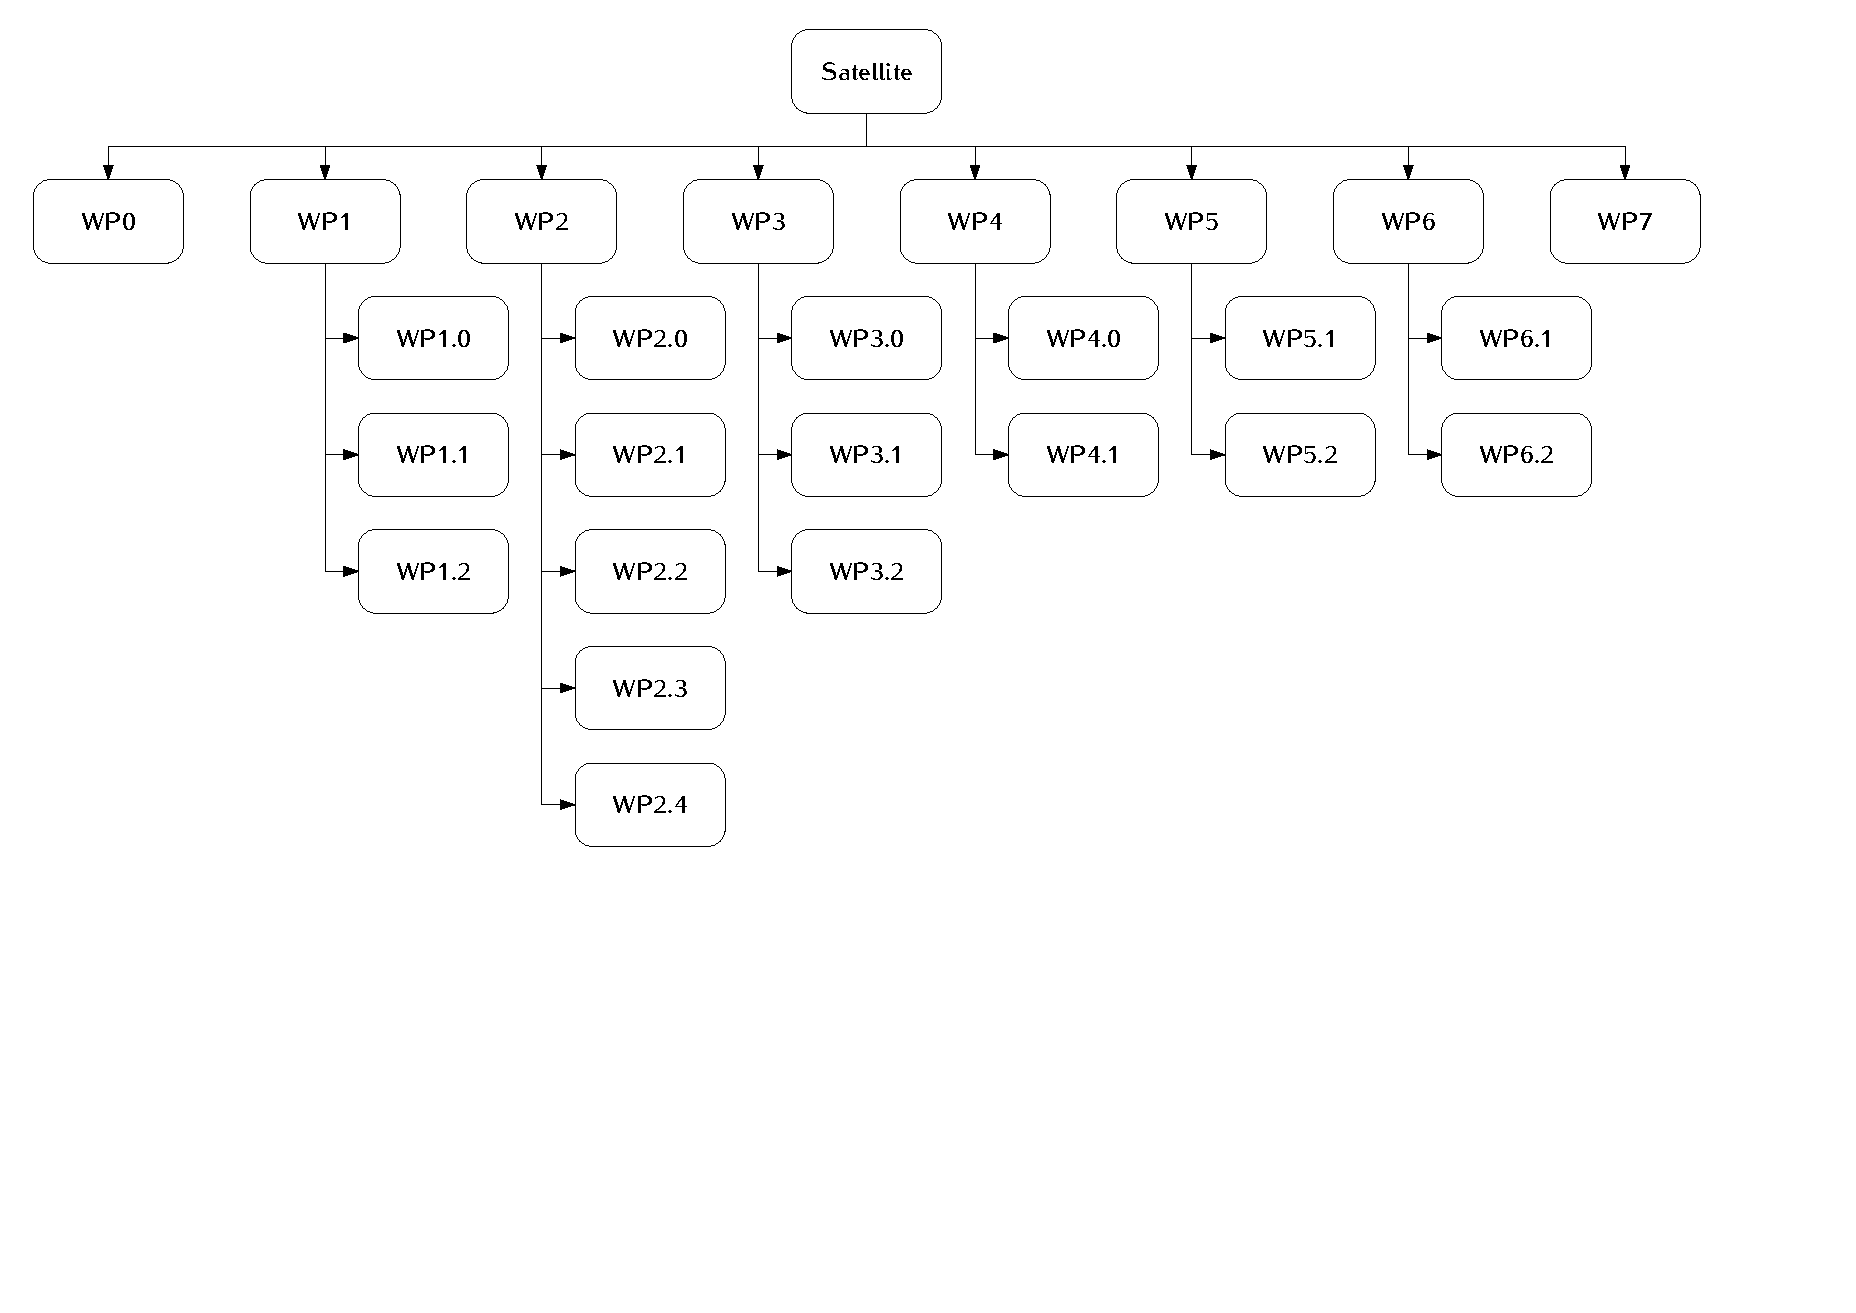
\includegraphics[width=\textwidth]{figures/wbs.pdf}
        \caption{WBS diagram.}
        \label{fig:wbs}
    \end{center}
\end{figure}

\begin{itemize}
    \item \textbf{WP0}: Management and preparation.
    \item \textbf{WP1}: Architecture study and specification.
        \begin{itemize}
            \item \textbf{WP1.0}: Operation scenario definition.
            \item \textbf{WP1.1}: Architecture definition.
            \item \textbf{WP1.2}: Requirements definition.
        \end{itemize}
    \item \textbf{WP2}: Engineering and flight models definition
        \begin{itemize}
            \item \textbf{WP2.0}: Application design.
            \item \textbf{WP2.1}: Platform design.
            \item \textbf{WP2.2}: Application implementation.
            \item \textbf{WP2.3}: Platform implementation.
            \item \textbf{WP2.4}: Decoder implementation (EGSE).
        \end{itemize}
    \item \textbf{WP3}: Engineering model integration.
        \begin{itemize}
            \item \textbf{WP3.0}: Subsystems integration and tests.
            \item \textbf{WP3.1}: Engineering model satellite integration.
            \item \textbf{WP3.2}: Integration and tests with decoder.
        \end{itemize}
    \item \textbf{WP4}: Engineering model validation.
        \begin{itemize}
            \item \textbf{WP4.0}: Validation scenarios specification.
            \item \textbf{WP4.1}: Project validation.
        \end{itemize}
    \item \textbf{WP5}: Fligth model integration.
        \begin{itemize}
            \item \textbf{WP5.0}: Subsystems integration and tests.
            \item \textbf{WP5.1}: Fligth model satellite integration.
        \end{itemize}
    \item \textbf{WP6}: Fligth model validation.
        \begin{itemize}
            \item \textbf{WP6.0}: Validation scenarios specification.
            \item \textbf{WP6.1}: Project validation.
        \end{itemize}
    \item \textbf{WP7}: Evaluation and dissemination.
\end{itemize}
